\documentclass[10pt,letterpaper]{article}

\usepackage[margin=0.55in]{geometry}
\usepackage{booktabs}
\usepackage{tabularx}
\usepackage{multirow}
\usepackage{graphicx}
\usepackage{caption}
\usepackage{subcaption}
\usepackage{tikz}
\usepackage{pgfplots}
\usepackage{hyperref}
\usepackage{xcolor}
\usepackage{enumitem}
\usepackage{titlesec}
\usepackage{microtype}
\usepackage[T1]{fontenc}
\usepackage{float}

\pgfplotsset{compat=1.18}
\usetikzlibrary{arrows.meta,positioning,fit,shapes.geometric}

\definecolor{bwcBlue}{HTML}{1F6F8B}
\definecolor{bwcCoral}{HTML}{B34D3A}
\definecolor{bwcGold}{HTML}{C58B2B}
\definecolor{bwcGray}{HTML}{4B5563}
\definecolor{bwcLight}{HTML}{EEF6F8}
\definecolor{bwcWarm}{HTML}{FFF3E8}

\hypersetup{
  colorlinks=true,
  linkcolor=bwcBlue,
  citecolor=bwcBlue,
  urlcolor=bwcBlue
}

\titlespacing*{\section}{0pt}{4pt}{1pt}
\titlespacing*{\subsection}{0pt}{3pt}{1pt}
\setlist[itemize]{leftmargin=*,nosep}
\setlength{\parindent}{0pt}
\setlength{\parskip}{1pt}
\captionsetup{font=small,labelfont=bf,skip=2pt}
\setlength{\textfloatsep}{6pt plus 1pt minus 2pt}
\setlength{\floatsep}{5pt plus 1pt minus 2pt}
\setlength{\intextsep}{5pt plus 1pt minus 2pt}

\newcommand{\pct}[1]{#1\%}
\newcommand{\code}[1]{\texttt{#1}}
\newcommand{\loss}[1]{\textcolor{bwcCoral}{#1}}

\title{\vspace{-2.5em}\textbf{BWC Adaptive Selector: Pair-Aware Runtime Prefetcher Selection in ChampSim}}
\author{Zhaofeng Luo \and Kijun Shin}
\date{15-740 Computer Architecture}

\begin{document}
\maketitle
\vspace{-1.4em}

\section*{0. Abstract}

Hardware prefetchers hide memory latency, but aggressive prefetch traffic can
consume shared cache capacity, memory queues, and off-chip bandwidth. This is
especially important in multicore systems, where a locally plausible prefetch
stream can delay demand requests from a peer. We address this prefetch-control
problem in ChampSim by building the BWC Adaptive Selector, a pair-aware L2
runtime selector over original SPP, an FDP-style SPP variant, and BOP. BWC uses
local stream features and peer/shared signals to decide whether the local expert
choice is safe under contention. Across Phase 1 scale sweeps at 1M+5M,
2M+10M, and 4M+20M, average gains remain positive for both single-core IPC
(\pct{+1.5464}, \pct{+1.8540}, \pct{+2.6782}) and two-core weighted speedup
(\pct{+1.3677}, \pct{+1.6013}, \pct{+1.3017}). Individual rows are mixed,
especially for some \code{lbm}-related pairs and near-neutral \code{bzip2} and
\code{lbm} single-core cases. OpenEvolve was then used in a focused Phase 2
2M+10M diagnostic to refine only pair coordination, improving
\code{bzip2 + lbm} and reducing the \code{mcf + lbm} worst-case loss. The main
insight is that prefetch control should be peer-aware: locally reasonable
prefetch decisions can become globally harmful under shared-resource contention.

\section*{1. Introduction}

Modern data prefetchers exploit regular memory behavior to fetch lines before
the core demands them. This can substantially improve performance for streaming
and structured workloads. However, prefetches are not free: each request
occupies queues, MSHRs, cache space, and DRAM bandwidth. In multicore systems,
these costs cross core boundaries. A prefetcher that helps one core locally can
hurt another core through shared LLC and memory-system pressure.

The project began from a bandwidth-aware control question: can a runtime policy
control an SPP-like prefetcher better than static or accuracy-only throttling?
Accuracy is useful but incomplete. A low-accuracy stream can still provide
coverage or memory-level effects, while a confident predictor can still create
harmful traffic. We therefore treat prefetching as a control problem, not only
an address-prediction problem.

The final artifact is the BWC Adaptive Selector. Rather than inventing a new
predictor, it chooses among experts with different behaviors: \code{spp\_orig},
\code{spp\_dev} with FDP-style controls, and \code{bop}. The selector asks two
questions on every stable window: what does the local stream look like, and
does the peer make the locally preferred choice risky? Our research question is
whether these local and peer/shared signals can choose safer prefetch behavior
than a single static policy. The scale sweep shows positive average behavior
over a static \code{SPP\_orig} baseline at all tested simulation lengths, while
also exposing fragility in individual cases. In particular, longer runs reveal
small regressions for several \code{lbm}-related pairs, so the final conclusion is
not that every case is solved; it is that peer-aware selection improves the
average tradeoff and points clearly to the remaining hard interactions.

\section*{2. Related Work}

Feedback Directed Prefetching (FDP) by Srinath et al. dynamically adjusts
prefetch aggressiveness using feedback such as accuracy, timeliness, and
pollution \cite{fdp}. Our \code{spp\_dev} expert contains an FDP-style
controller, but the final design builds above it: it selects among experts and
uses pair signals to avoid choices that are unsafe under shared contention.

The Signature Path Prefetcher (SPP), based on path-confidence lookahead
prefetching, is our main SPP baseline \cite{spp}. It uses signatures and
confidence to look ahead in access streams. Best-Offset Prefetching (BOP)
searches for spatial offsets that work for the current stream \cite{bop}. In
our design, these mechanisms are not only baselines but also expert behaviors:
SPP represents the strong default lookahead prefetcher, the FDP-style variant
represents a feedback-controlled SPP mode, and BOP represents an offset-oriented
alternative for streams where it behaves differently. BWC differs by adding a
selector and pair coordinator above the experts rather than replacing their
address-generation logic. ChampSim is the trace-based simulation framework used
to evaluate these designs \cite{champsim}. OpenEvolve is an evolutionary coding
framework with LLM-guided mutation and quality-diversity search
\cite{openevolve}. We use it in a narrow, coordinator-only way so the evolved
design remains interpretable.

\section*{3. Method}

\subsection*{Implementation Overview}

The main implementation is in \code{prefetcher/adaptive\_selector/}. The
Phase 2 retained best point is stored separately in
\code{prefetcher/adaptive\_selector\_phase2\_best/}. Table~\ref{tab:impl}
maps the main selector stages to source-level artifacts.

\begin{table}[!htbp]
\centering
\scriptsize
\caption{Source artifacts and implementation map.}
\label{tab:impl}
\begin{tabularx}{\linewidth}{@{}p{0.20\linewidth}p{0.25\linewidth}X@{}}
\toprule
Stage & Main function / artifact & Role \\
\midrule
Feature extraction & \code{compute\_window\_features()} & Computes \code{page\_growth}, \code{line\_growth}, \code{small\_delta\_ratio}, and \code{rfo\_share}. \\
Local selection & \code{classify\_window()} & Produces the local \code{orig}, \code{FDP}, or \code{BOP} candidate. \\
Shared context & \code{refresh\_shared\_pressure()} & Records local pressure plus peer page/delta signatures and \code{peer\_lbm\_like}. \\
Pair coordination & \code{coordinate\_candidate()} & Remaps or blocks risky pair choices before activation. \\
Configurations & \code{adaptive\_selector} configs & Instantiate the selector in single-core and two-core ChampSim runs. \\
\bottomrule
\end{tabularx}
\end{table}

\begin{figure}[t]
\centering
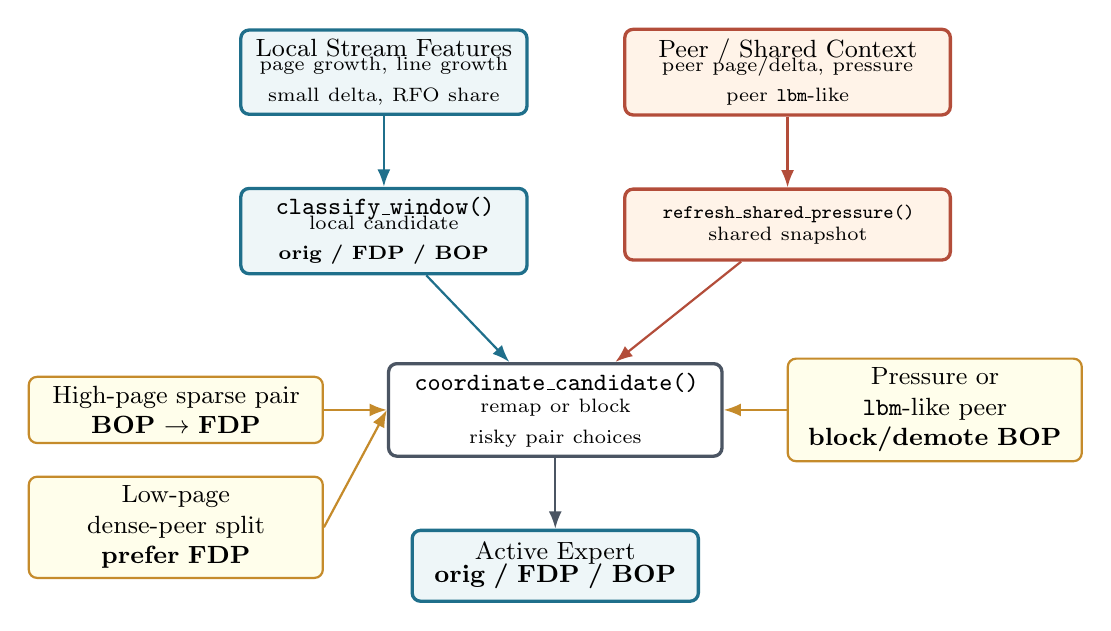
\begin{tikzpicture}[
  font=\small,
  node distance=9mm and 12mm,
  box/.style={draw=bwcBlue, rounded corners=3pt, very thick, fill=bwcLight, align=center, minimum height=9mm, text width=34mm},
  peer/.style={draw=bwcCoral, rounded corners=3pt, very thick, fill=bwcWarm, align=center, minimum height=9mm, text width=39mm},
  coord/.style={draw=bwcGray, rounded corners=3pt, very thick, fill=white, align=center, minimum height=10mm, text width=40mm},
  rule/.style={draw=bwcGold, rounded corners=3pt, thick, fill=yellow!8, align=center, text width=35mm, minimum height=8mm},
  arrow/.style={-{Latex[length=2.2mm]}, thick}
]
\node[box] (features) {Local Stream Features\\[-1mm]\scriptsize page growth, line growth\\small delta, RFO share};
\node[peer, right=of features] (peerctx) {Peer / Shared Context\\[-1mm]\scriptsize peer page/delta, pressure\\peer \code{lbm}-like};
\node[box, below=of features] (classify) {\code{classify\_window()}\\[-1mm]\scriptsize local candidate\\\textbf{orig / FDP / BOP}};
\node[peer, below=of peerctx] (refresh) {\scriptsize\code{refresh\_shared\_pressure()}\\[-1mm]\scriptsize shared snapshot};
\node[coord, below right=11mm and -18mm of classify] (coord) {\code{coordinate\_candidate()}\\[-1mm]\scriptsize remap or block risky pair choices};
\node[box, below=of coord] (active) {Active Expert\\[-1mm]\textbf{orig / FDP / BOP}};

\draw[arrow,bwcBlue] (features) -- (classify);
\draw[arrow,bwcCoral] (peerctx) -- (refresh);
\draw[arrow,bwcBlue] (classify) -- (coord);
\draw[arrow,bwcCoral] (refresh) -- (coord);
\draw[arrow,bwcGray] (coord) -- (active);

\node[rule, left=8mm of coord] (r1) {High-page sparse pair\\\textbf{BOP $\rightarrow$ FDP}};
\node[rule, below=4mm of r1] (r2) {Low-page dense-peer split\\\textbf{prefer FDP}};
\node[rule, right=8mm of coord] (r3) {Pressure or \code{lbm}-like peer\\\textbf{block/demote BOP}};
\draw[arrow,bwcGold] (r1.east) -- (coord.west);
\draw[arrow,bwcGold] (r2.east) -- (coord.west);
\draw[arrow,bwcGold] (r3.west) -- (coord.east);
\end{tikzpicture}
\caption{Simplified BWC Adaptive Selector pipeline, based on the poster flow. Local stream features select a candidate; peer/shared signals guard the final activation.}
\label{fig:pipeline}
\end{figure}

Figure~\ref{fig:pipeline} shows the final design. Each demand access is pushed
into a sliding window, and the window produces four local features. A local
classifier proposes an expert. In two-core mode, shared snapshots record peer
behavior and pressure. The coordinator then applies pair-aware rules before the
candidate becomes the active expert. We use the name FDP for the FDP-style SPP
expert in the selector; it is not a full reimplementation of the FDP paper, but
an SPP variant with feedback-style controls intended to be safer under some
traffic patterns. Overall, the simulated policy is relatively
hardware-conscious: it relies on short counters, ratios, threshold comparisons,
and a small shared state vector rather than expensive global history.

\subsection*{OpenEvolve Setup}

The original proposal planned a parameter-only OpenEvolve search over an SPP
controller. During development, the retained artifact shifted to expert
selection because it gave clearer control over heterogeneous pair behavior.
For Phase 2, OpenEvolve searched only the coordinator logic. The expert
prefetchers stayed fixed. The best retained point changed several pair
fallbacks from \code{orig} to FDP, including dense-peer split handling,
pair-scope BOP demotion, and \code{lbm}-like peer protection. It also added two
runtime guards for sparse/high-page-growth cores paired with \code{lbm}-like
peers, and for \code{lbm}-like cores paired with high-page-growth peers.

For OpenEvolve, we constrained mutations to the pair-coordination decision path,
primarily \code{coordinate\_candidate()}, and kept the expert prefetchers and
ChampSim interfaces fixed. The prompt emphasized preserving the Phase 1
selector behavior while improving fragile \code{lbm}-related pair cases. Each
candidate was evaluated on a focused 2M-warmup plus 10M-simulation mini-suite
containing single-core \code{lbm}, \code{bzip2 + lbm}, and \code{mcf + lbm}. The
score combined mean gain with a worst-case guardrail so that a candidate had to
improve pair behavior without introducing a new large regression. We retained
the best candidate according to this focused score and report the broader final
performance summary separately. The reported combined score is this internal
OpenEvolve ranking objective; higher is better, and it is used only to rank
Phase 2 candidates rather than as a separate architectural metric.

\newpage
\subsection*{Evaluation Setup}

\begin{center}
\small
\captionsetup{hypcap=false}
\captionof{table}{Evaluation setup.}
\label{tab:setup}
\begin{tabularx}{\linewidth}{@{}p{0.22\linewidth}X@{}}
\toprule
Item & Setting \\
\midrule
Simulator & ChampSim trace-based simulation. \\
Primary baseline & \code{SPP\_orig}; reported gains are relative to this baseline. \\
Selector configs & \code{configs/adaptive\_selector\_config.json} and \code{configs/adaptive\_selector\_2core.json}. \\
Experts & Original SPP, FDP-style SPP, and BOP. \\
Workloads & \code{astar}, \code{mcf}, \code{lbm}, and \code{bzip2}. \\
Metrics & Single-core IPC and two-core weighted speedup. \\
Weighted-speedup definition & Sum of each core's shared-run IPC normalized to its corresponding single-core IPC; gains are relative to the \code{SPP\_orig} pair baseline. \\
Phase 1 scale sweep & \code{1M+5M}, \code{2M+10M}, and \code{4M+20M}; baseline is \code{spp\_orig}, current is phase 1 final \code{adaptive\_selector}. \\
Sweep execution & Completed on \code{office-kijun} with at most 3 sweep jobs in parallel. \\
Phase 2 run length & 2M warmup plus 10M simulation for the focused OpenEvolve comparison. \\
\bottomrule
\end{tabularx}
\end{center}

\section*{4. Experimental Results}

\noindent\textbf{Phase 1 scale sweep.}
The main final result is a scale sweep of the Phase 1 final selector against
\code{spp\_orig}. Table~\ref{tab:scaleavg} and Figure~\ref{fig:scaleavg} show
that average single-core and two-core gains stay positive at all three tested
lengths. The averages hide important variation, so Tables~\ref{tab:singlematrix}
and~\ref{tab:pairmatrix} report the per-workload and per-pair gain matrices.

\begin{table}[H]
\centering
\scriptsize
\caption{Phase 1 final scale sweep average gains.}
\label{tab:scaleavg}
\begin{tabular}{@{}lrr@{}}
\toprule
Scale & Single-core average IPC gain & Two-core average WS gain \\
\midrule
\code{1M+5M} & \pct{+1.5464} & \pct{+1.3677} \\
\code{2M+10M} & \pct{+1.8540} & \pct{+1.6013} \\
\code{4M+20M} & \pct{+2.6782} & \pct{+1.3017} \\
\bottomrule
\end{tabular}
\end{table}

\begin{figure}[H]
\centering
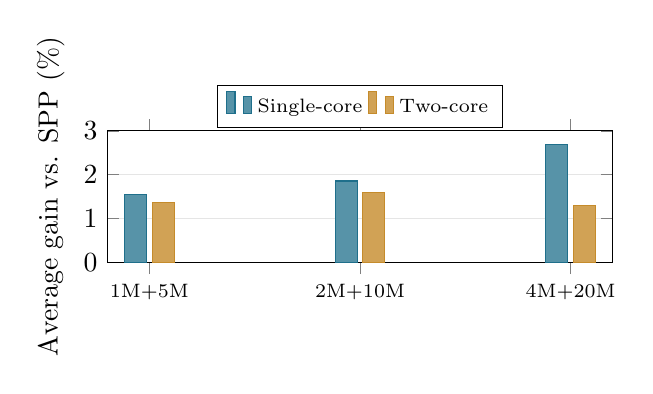
\begin{tikzpicture}
\begin{axis}[
  ybar,
  width=0.66\linewidth,
  height=3.25cm,
  ymin=0,
  ymax=3.0,
  bar width=8pt,
  ylabel={Average gain vs. SPP (\%)},
  symbolic x coords={1M+5M,2M+10M,4M+20M},
  xtick=data,
  x tick label style={font=\scriptsize},
  legend style={font=\scriptsize, at={(0.5,1.02)}, anchor=south, legend columns=2},
  ymajorgrids=true,
  grid style={draw=gray!20}
]
\addplot[fill=bwcBlue!75, draw=bwcBlue] coordinates {(1M+5M,1.5464) (2M+10M,1.8540) (4M+20M,2.6782)};
\addplot[fill=bwcGold!80, draw=bwcGold] coordinates {(1M+5M,1.3677) (2M+10M,1.6013) (4M+20M,1.3017)};
\legend{Single-core, Two-core}
\end{axis}
\end{tikzpicture}
\caption{Scale-sweep average gains. Average behavior remains positive, but the detailed matrices show that several individual cases are still fragile.}
\label{fig:scaleavg}
\end{figure}

\begin{table}[!htbp]
\centering
\scriptsize
\caption{Single-core IPC gain matrix for the Phase 1 final selector.}
\label{tab:singlematrix}
\begin{tabular}{@{}lrrr@{}}
\toprule
Workload & \code{1M+5M} & \code{2M+10M} & \code{4M+20M} \\
\midrule
\code{astar} & \pct{+2.6292} & \pct{+3.8644} & \pct{+5.9008} \\
\code{mcf} & \pct{+3.7178} & \pct{+3.1798} & \pct{+4.8350} \\
\code{lbm} & \loss{\pct{-0.0708}} & \pct{+0.3722} & \loss{\pct{-0.0165}} \\
\code{bzip2} & \loss{\pct{-0.0907}} & \loss{\pct{-0.0006}} & \loss{\pct{-0.0066}} \\
\bottomrule
\end{tabular}
\end{table}
The single-core sweep is strongest on \code{astar} and \code{mcf}; \code{lbm}
and \code{bzip2} are near-neutral and sometimes slightly negative. This suggests
the selector's local feature rules help irregular/memory-sensitive workloads
more reliably than already-stable dense or compute-heavy streams.

\begin{table}[!htbp]
\centering
\scriptsize
\caption{Two-core weighted-speedup gain matrix. Negative entries are highlighted.}
\label{tab:pairmatrix}
\begin{tabular}{@{}lrrr@{}}
\toprule
Pair & \code{1M+5M} & \code{2M+10M} & \code{4M+20M} \\
\midrule
\code{mcf + astar} & \pct{+2.6541} & \pct{+4.3939} & \pct{+4.6815} \\
\code{astar + bzip2} & \pct{+1.5328} & \pct{+2.2457} & \pct{+2.7770} \\
\code{bzip2 + mcf} & \pct{+1.3779} & \pct{+2.1973} & \pct{+1.2700} \\
\code{astar + lbm} & \pct{+1.4340} & \pct{+1.3858} & \loss{\pct{-0.1283}} \\
\code{bzip2 + lbm} & \pct{+0.5820} & \loss{\pct{-0.0286}} & \loss{\pct{-0.1448}} \\
\code{mcf + lbm} & \loss{\pct{-0.1211}} & \loss{\pct{-1.0157}} & \loss{\pct{-0.6557}} \\
\code{astar + astar} & \pct{+4.2142} & \pct{+4.9374} & \pct{+4.1861} \\
\code{mcf + mcf} & \pct{+1.7809} & \pct{+1.8082} & \pct{+1.1320} \\
\code{lbm + lbm} & \pct{+0.1705} & \pct{+0.0706} & \loss{\pct{-0.1168}} \\
\code{bzip2 + bzip2} & \pct{+0.0515} & \pct{+0.0187} & \pct{+0.0155} \\
\bottomrule
\end{tabular}
\end{table}
The two-core averages remain positive, but longer runs expose the hard cases:
\code{mcf + lbm} is negative at every scale, and several other \code{lbm} pairs
turn negative at 4M+20M. This is the clearest evidence that peer-aware control
is useful but incomplete.

\noindent\textbf{Phase 2 OpenEvolve diagnostic.}
Phase 2 is a focused 2M+10M diagnostic rather than a replacement for the scale
sweep. It targets the fragile \code{lbm} cases exposed by the sweep. The best
candidate changes only \code{coordinate\_candidate()} and improves the two
target pair summaries, as shown in Table~\ref{tab:phase2} and
Figure~\ref{fig:phase2gains}.

\begin{table}[!htbp]
\centering
\scriptsize
\caption{Phase 2 OpenEvolve best point.}
\label{tab:phase2}
\begin{tabular}{@{}lrrrrrr@{}}
\toprule
Case & SPP base & Phase 1 & P1 gain & Phase 2 & P2 gain & Delta \\
\midrule
\code{lbm} IPC & 0.866441 & 0.869666 & \pct{+0.3722} & 0.869666 & \pct{+0.3722} & +0.0000 pp \\
\code{bzip2 + lbm} WS & 1.792235 & 1.791723 & \pct{-0.0286} & 1.793705 & \pct{+0.0820} & +0.1106 pp \\
\code{mcf + lbm} WS & 1.256300 & 1.243540 & \pct{-1.0157} & 1.249503 & \pct{-0.5410} & +0.4747 pp \\
\bottomrule
\end{tabular}
\end{table}

\begin{figure}[!htbp]
\centering
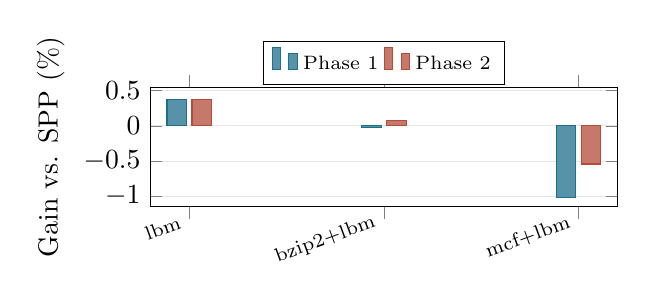
\begin{tikzpicture}
\begin{axis}[
  ybar,
  width=0.62\linewidth,
  height=3.1cm,
  ymin=-1.15,
  ymax=0.55,
  bar width=7pt,
  ylabel={Gain vs. SPP (\%)},
  symbolic x coords={lbm,bzip2+lbm,mcf+lbm},
  xtick=data,
  x tick label style={font=\scriptsize, rotate=20, anchor=east},
  legend style={font=\scriptsize, at={(0.5,1.02)}, anchor=south, legend columns=2},
  ymajorgrids=true,
  grid style={draw=gray!20}
]
\addplot[fill=bwcBlue!75, draw=bwcBlue] coordinates {(lbm,0.3722) (bzip2+lbm,-0.0286) (mcf+lbm,-1.0157)};
\addplot[fill=bwcCoral!75, draw=bwcCoral] coordinates {(lbm,0.3722) (bzip2+lbm,0.0820) (mcf+lbm,-0.5410)};
\legend{Phase 1, Phase 2}
\end{axis}
\end{tikzpicture}
\caption{Phase 2 before/after gains. OpenEvolve fixes the small \code{bzip2 + lbm} regression and reduces the \code{mcf + lbm} loss from \pct{-1.0157} to \pct{-0.5410}.}
\label{fig:phase2gains}
\end{figure}

The aggregate internal ranking score improves from -6.2665 to -3.0105, where
higher is better. Mean gain improves by 0.1951 percentage points and worst-case
gain by 0.4747 percentage points.

\noindent\textbf{Experimental process.}
The process was iterative: local selection produced useful wins, pair-aware
coordination protected several mixed workloads, the scale sweep exposed
remaining \code{lbm} fragility, and Phase 2 used coordinator-only OpenEvolve
mutations to reduce those failures.

\begin{table}[!htbp]
\centering
\scriptsize
\caption{Experimental progression leading to the final report state.}
\label{tab:process}
\begin{tabularx}{\linewidth}{@{}p{0.24\linewidth}X@{}}
\toprule
Stage & What it established \\
\midrule
Sliding-window selector & Local stream features could choose among \code{orig}, FDP, and BOP without changing expert internals. \\
Pair-aware coordination & Some locally plausible choices were harmful under shared pressure, especially when an \code{lbm}-like peer was present. \\
Scale sweep & Average gains remained positive at \code{1M+5M}, \code{2M+10M}, and \code{4M+20M}, but individual \code{lbm} pairs exposed stability limits. \\
OpenEvolve Phase 2 & Coordinator-only mutations improved the focused \code{bzip2 + lbm} and \code{mcf + lbm} diagnostics without changing expert predictors. \\
\bottomrule
\end{tabularx}
\end{table}

\section*{5. Goals and Next Steps}

The original proposal goal was an OpenEvolve-optimized bandwidth-aware SPP
controller. We partially met that goal, but the final artifact shifted to a
stronger adaptive-selector formulation. Instead of tuning a single SPP
controller, we select among SPP, FDP-style SPP, and BOP. This better matches
the observed problem: different workloads and pairs need different expert
styles, not only different throttling thresholds. Although this shift changed
the mechanism, it preserved the proposal's larger goal: using automated search
to improve prefetch control under shared-resource pressure.

Future work should evaluate more held-out SPEC mixes, run longer and repeated
simulations, validate four-core behavior, and use OpenEvolve over a broader
but still constrained coordinator rule space. The scale sweep makes the most
useful next analysis clear: ablate each pair rule and report prefetch traffic,
cache pollution, and queue pressure alongside IPC and weighted speedup.

\section*{6. Collaboration}

Zhaofeng Luo focused on experiment infrastructure, running ChampSim
evaluations, collecting IPC and weighted-speedup summaries, and preparing the
final result tables and poster figures. He also led the final report and poster
writing, helped analyze the single-core and two-core results, and validated the
retained result ledger.

Kijun Shin focused on the adaptive-selector implementation, pair-coordination
rules, and OpenEvolve-guided Phase 2 refinement. He also helped debug the
coordinator behavior and interpret the evolved changes to
\code{coordinate\_candidate()}.

Both members jointly designed the BWC selector idea, studied related
prefetching work, discussed evaluation methodology, reviewed intermediate
results, and refined the final project narrative.

\section*{7. Conclusion}

The BWC Adaptive Selector demonstrates that prefetch control should not be
purely local. The selector uses local stream features to choose an expert and
peer/shared signals to decide whether that choice is safe for the memory
system. The scale sweep shows positive average gains at all tested lengths, but
also exposes remaining fragility in individual \code{lbm}-related cases. The
Phase 2 OpenEvolve best point further shows that narrow, coordinator-only
evolution can reduce those difficult interactions without changing expert
predictor internals. The central lesson is simple: the right prefetcher for one
core is not always the right prefetcher for the system.

\enlargethispage{3\baselineskip}
\small
\begin{thebibliography}{9}
\bibitem{fdp}
S. Srinath, O. Mutlu, H. Kim, and Y. N. Patt. Feedback Directed Prefetching:
Improving the Performance and Bandwidth-Efficiency of Hardware Prefetchers.
HPCA, 2007. \url{https://hps.ece.utexas.edu/pub/srinath_hpca07.pdf}

\bibitem{spp}
J. Kim, S. H. Pugsley, P. V. Gratz, A. L. N. Reddy, C. Wilkerson, and
Z. Chishti. Path Confidence Based Lookahead Prefetching. MICRO, 2016.
\url{https://dblp.org/rec/conf/micro/KimPGRWC16.html}

\bibitem{bop}
P. Michaud. Best-Offset Hardware Prefetching. HPCA, 2016.
\url{https://core.ac.uk/outputs/48160133/}

\bibitem{champsim}
N. Gober, G. Chacon, L. Wang, P. V. Gratz, D. A. Jimenez, E. Teran,
S. H. Pugsley, and J. Kim. The Championship Simulator: Architectural Simulation
for Education and Competition. arXiv:2210.14324, 2022.
\url{https://arxiv.org/abs/2210.14324}

\bibitem{openevolve}
OpenEvolve project repository.
\url{https://github.com/algorithmicsuperintelligence/openevolve}. Accessed Apr. 2026.
\end{thebibliography}

\end{document}
